\documentclass[10pt]{article}

% \setcitestyle{numbers}
\usepackage[numbers]{natbib}
\usepackage[english]{babel}
\usepackage[utf8x]{inputenc}
\usepackage{amsmath}
\usepackage{graphicx}
\usepackage{longtable}
\usepackage[]{hyperref}
\usepackage{comment}
\usepackage{xspace}
\usepackage[usenames]{color}
\usepackage{datetime}
\usepackage{bm}

\title{Measurement of Blended Objects in LSST\\
{\author{
    Jim Bosch\\
    {\em for LSST Data Management}
}}}

\begin{document}

\maketitle

\section{Introduction}

Most LSST objects will overlap one or more of its neighbors enough to affect
naive measurements of their properties.  One of the major challenges in the
deep processing pipeline will be measuring these sources in a way that
corrects for and/or characterizes the effect of these blends.

The measurements of interest can be split up broadly into two categories:
\begin{itemize}
    \item weighted moments (includes aperture fluxes and most centroiders)
    \item forward modeling
\end{itemize}

Most measurements that involve the PSF or a PSF-convolved function as a weight
function can be interpreted in either way, but must be treated as weighted
moments in calculating their uncertainties (i.e. per-pixel variances must
not be used in the weighting) in order to produce unbiased fluxes.

The statistical framework in which weighted moments make sense assumes that
each object is isolated from its neighbors.  As a result, our only option for
these measurements is {\em deblending}, which we define here as any
procedure that attempts to remove neighbors from the pixel values prior to
measurement.

In forward modeling, we convolve a model for the object with our model for
the PSF, compare this model to the data, and either optimize to find
best-fit parameters or explore the full likelihood surface in another way
(e.g. Monte Carlo sampling).  We can use the deblending approach for
forward fitting, simply by fittting each object separately to the deblended
pixels.  However, we can also use {\em simultaneous fitting}, in which we
optimize or sample the models for multiple objects jointly.

Both deblending and simultaneous fitting have some advantages and
disadvantages:
\begin{itemize}
\item Deblending provides no direct way to characterize the uncertainties in
      an object's measurements due to neighbors, while these are naturally
      captured in the full likelihood distribution of a simultaneous fit.
      This likelihood distribution may be very high-dimensional in a fit that
      involves many objects, however, and may be difficult to characterize or
      store.
\item Deblending generally allows for more flexible morphologies than the
      analytic models typically used in forward fitting, which is particularly
      important for nearby galaxies and objects blended with them;
      simultaneous fitting is only statistically well-motivated to the extent
      the models used can reproduce the data.
\item Once deblended pixels are available, fitting objects simultaneously will
      almost always be more computationally expensive than fitting them
      separately to the deblended pixels.  At best, simultaneous fitting will
      have similar performance but still require more complex code.  And
      because we will need to deblend pixels to support some measurement
      algorithms, we'll always have to deblend whether we want to subsequently
      do simultaneous fitting or not.
\end{itemize}

This paper focuses on the problem of blended measurement only; the details of
how we deblend pixels and the models and algorithms we use in simultaneous
fitting will be described elsewhere.

\section{Blend Families and Footprints}

We identify groups of blended objects at the detection stage from their
isophotes at the detection limit; a single simply-connected region of
above-threshold pixels is a {\em parent}, with {\em children} initially
discovered as peaks within that region.  These peaks may not originate in
the same image; we will merge peaks from multiple detection images (e.g.
coadds of different filters or ranges of observation dates).

We call the above-threshold region (and the data structure that defines it) a
\texttt{Footprint}, and the combination of such a region with the values of
the pixels within it (either original data or deblended) a \texttt
{HeavyFootprint}.

For each blend family, in addition to measuring the properties of the children
(either via deblending or simultaneous fitting), we also measure the parent:
we interpret the region as a single unblended object. This is essentially
an incomplete but useful hedge against overdeblending (we'd like to evaluate
all alternate hypotheses for any combination of peaks belonging to the same
object, but that's infeasible).

\section{Deblended Measurement}

\label{sec:deblender}

The specific approach to deblending we plan to take for LSST is based on
the deblender in the SDSS {\em Photo} pipeline.

Given pixel values $I_{i}$, we create a ``template'' $T_{i,j}$ that represents
an attempt to model the surface brightness of object $j$ at pixel
$i$.\footnote {
    In {\em~Photo}, this template was determined from symmetry arguments and a
    number of heuristics; a full description of how we plan to generate
    templates in LSST is beyond the scope of this paper.
}  We then find the best least-squares linear combination of templates to the
data (ignoring per-pixel variances), solving for coefficients $\alpha_{j}$:
\begin{align}
\bm{\alpha} = \left(\bm{T}^T\bm{T}\right)^{-1}\!\bm{T}^T\bm{I}
\end{align}
Our best-fit prediction for the pixel value vector is thus
$\bm{T}\bm{\alpha}$.
Because this is not the same as the true pixel vector $\bm{I}$, we do not use
the per-object model prediction $\bm{T}\bm{\alpha}$ directly for the deblended
pixel values; instead we reapportion the true per-pixel fluxes according to
the relative predicted contribution from each object:
\begin{align}
D_{i,j} = \frac{
    T_{i,j} \, \alpha_j
}{
    \sum\limits_k T_{i,k} \, \alpha_k
}
I_i
\end{align}

While these deblended pixel values $D_{i,j}$ are what we store in the
\texttt{HeavyFootprint} for each child object, we do not perform measurements
on these values directly for two reasons:
\begin{itemize}
\item $D_{i,j}$ typically has many zero entries, especially for a large blend
    family (i.e. many pixels for which a particular object has no
    contribution).  We include only the nonzero values in the
    \texttt{HeavyFootprint}s for efficiency reasons.
\item Many measurements utilize pixels beyond the blend family's
    \texttt{Footprint}, and in fact may extend to pixels that are in another
    family.
\end{itemize}
To address these issues, we measure deblended objects using the following
procedure:
\begin{enumerate}
\item Replace every above threshold pixel in the image (all
    \texttt{Footprint}s) with randomly generated noise that matches
    the background noise in the image.
\item For each blend family:
    \begin{enumerate}
    \item For each child object in the current blend family:
        \begin{enumerate}
        \item Insert the child's \texttt{HeavyFootprint} into the image,
            replacing (not adding to) any pixels it covers.
        \item Run all measurement algorithms to produce {\em child}
            measurements.
        \item Replace the pixels in the child's \texttt{Footprint} region
            with (the same) random noise again.
        \end{enumerate}
    \item Revert the pixels in the parent \texttt{Footprint} to their original
        values.
    \item Run all measurement algorithms to produce {\em parent} measurements.
    \item Replace the parent \texttt{Footprint} pixels with (the same) random
        noise again.
    \end{enumerate}
\end{enumerate}
This procedure double-counts flux that is not part of a \texttt{Footprint},
but this is considered better than ignoring this flux, because most
measurement algorithms utilize some other procedure for downweighting the
contribution of faraway pixels.

\section{Simultaneous Fitting}

\subsection{Model Selection}

\label{sec:model-selection}

The LSST pipeline will fit both a moving point source and a galaxy model to
each object.  With simultaneous fitting, however, we also have to consider
which models to use for neighbors, and it is clear that allowing for every
possible combination is infeasible (we'd need to fit each blend $2^N$ times,
where $N$ is the number of objects in the blend).

One possible alternative would be to determine the best model for each
object from separate fitting done on deblended pixels, and then fit
simultaneously using just those models.  This makes the simultaneous fitting
essentially useless for classification purposes, however, and it doesn't
reflect the reality that many objects will be impossible to securely classify.

Another option would be to do a single simultaneous fit using a hybrid model
that transitions between a moving point source and a galaxy model.  Because
a non-moving point source is a limit shared by both models, the transition is
continuous, and it should be possible to fit using both sampling methods and
optimization algorithms with some modification (though it will probably be
impossible to use general-purpose algorithms without modification, given the
complexity of the parameter constraints).

\subsection{Minimization}

Simultaneous fitting using optimization algorithms is straightforward from a
mathematical standpoint, but potentially difficult from a computational and
storage standpoint.

Nearly all numerical optimization algorithms involve a matrix factorization
for which the computation complexity is $O(N^2)$ in the number of parameters,
and this makes the worst-case performance scale with the square of the number
of objects in the blend (since the number of total parameters scales linearly
with the number of objects being fit together).  This matrix is typically
sparse for extremely large blends, so sparse matrix methods may avoid this
problem (at an additional cost in overhead).  It is also worth noting that
while the limiting performance for extremely large blends may go as $O(N^2)$,
the bottleneck in fitting galaxies is generally the evaluation of the
models and their first derivatives, which is just $O(N)$ in the number of
parameters.

Optimization-based fitting typically includes an estimate of the parameter
covariance matrix as one of its outputs, and in simultaneous fitting this
covariance matrix naturally includes cross-object terms.  These terms are, of
course, how we characterize how our uncertainty of an object's properties is
affected by its neighbors, and hence are in some sense the reason we're doing
simultaneous fitting at all.  These terms don't fit naturally within the
usual catalog/database model, in which one row corresponds to a single object.
The cross-object terms would need to be stored in some other way, making them
more difficult for users to access.  Perhaps more importantly, for large
blends the total number of outputs is $O(N^2)$ in the number of objects.  The
matrix should be sparse for sufficiently large blends, however, so a storage
scheme that takes advantage of this would address the problem.

If we elect to use hybrid models described in \ref{sec:model-selection}, we
will almost certainly have to develop our own optimization code rather than
adopt an existing third-party code.  High-quality optimization libraries that
can handle complex parameter constraints are extremely rare, and generally
focused on a very specific domain.  It is likely we'd have to develop our own
optimizer even for single-object, non-simultaneous fitting, however, as even
the simpler constraints involved in a single-object galaxy models are
sufficiently complex to give most free optimizers trouble.

\subsection{Monte Carlo Sampling}

\label{sec:sampling}

One of the advantages of Monte Carlo methods is that they scale better than
optimization methods as dimensionality increases.  If we consider the samples
themselves to be the output of such an algorithm, the storage and catalog
problems we encountered for optimizer outputs simply don't occur: if we sample
simultaneously from a multi-object posterior, we can simply split the storage
and representation of those samples across objects: they'll be the same
samples, but each object's storage will only include its own parameters.
Taken together, the samples represent the joint posterior for all objects in
a blend; taken separately, they represent the marginal posteriors.

The scaling with dimensionality for most Markov Chain Monte Carlo algorithms
depends strongly on the nature of the distribution itself.  The burn-in period
for such algorithms is typically thousands of samples, however, which makes
them impractical for our problem, for which we can only evaluate approximately
200 samples per object (at least when fitting to multi-epoch data).  Instead,
our baseline plan is to use adaptive importance sampling, in which we draw
samples from an analytic distribution that we construct to approximate the
true distribution, then weight those samples according to the true
distribution.  We can then use those weighted samples to modify the analytic
distribution in an iterative sense.  Most importantly, we can do most of these
iterations using a fast approximation to the true likelihood (by fitting to a
coadd instead of multiple epochs, or using a fast but inexact convolution).

Unfortunately, this means we need to construct, draw from, and update
a high-dimensional analytic distribution (typically a mixture Gaussians or
Student's T), and these operations are typically $O(N^2)$ in the total number
of parameters.  As with optimizers, these operations are nearly always
subdominant to the time required to evaluate the likelihood itself.  Instead,
it is the potential complexity of the likelihood surface for large blends that
is most concerning, especially when hybrid models are considered.  In
principle, anything can be done with mixture distributions, but it remains an
open question how efficient this approach will be.

\section{Divide and Conquer for Large Blends}

Regardless of the efficiency of our algorithms in the large-blend limit, it
will be necessary to split the very largest blends and handle them
iteratively.   This will happen automatically, of course, at the boundaries
of our sky pixellization scheme, as some blends will inevitably land on the
boundary between sky patches.  This can be handled straightforwardly by
defining overlapping patches, so that objects near the boundary are processed
twice (once with each patch).  One patch's processing is then selected to
be canonical on an object-by-object basis.  For successful deblending, this
approach essentially relies on individual objects landing entirely within one
patch, along with enough of any neighbors to deblend the primary object.

This requirement will not be met for some large galaxies (or pairs of large
galaxies), and we'll likely have to use a different algorithm for these.  The
same may be true for some extremely large blends that do fit entirely within
one patch, if necessary to keep deblender compute resources minimal.  A multi-
scale approach seems natural here - start on a binned image of a larger sky
area, and use this to generate templates for the largest objects.  We then
move to subimages at high resolution resolution to produce templates for
smaller object, until we return to the regular pixel scale. The final linear
fit for template coeffients ($\bm{\alpha}$) could then be done on a
combination of regular pixels and binned superpixels, depending on which
templates are active in a particular region, and may make use of sparse matrix
methods.  This approach may need to be iterative.

We may or may not want to use the same divisions for simultaneous fitting.  By
the time we reach the simultaneous fitting stage, we'll have some idea of the
extents of children, and we may be able to find a divisions that require
smaller overlap regions and/or a smaller number of objects with duplicate
processing (by drawing boundaries that only touch a small number of compact
objects). Patch boundaries will also be less important, as we'll be able to
iterate directly over blend families (and hence only worry about sky patches
for I/O).  It may even be unnecessary to do any kind of divide-and-conquer for
simultaneous fitting if we use sparse matrix methods and parallelize in a way
that splits likelihood evaluation over multiple cores.

\section{Models as Deblend Templates}

\label{sec:models-as-templates}

Thus far we've considered simultaneous fitting as an optional stage following
per-pixel deblending.  We can also use the results of a simultaneous fit as
the weighted templates ($\bm{T}\bm{\alpha}$) in a subsequent deblending step.

We've already highlighted model flexibility as an advantage of deblended
measurement over simultaneous fitting, and this approach would remove
some of that advantage, because the models used in simultaneous fitting are
not as flexible as {\em e.g.} SDSS-style templates derived from symmetry
arguments.  It wouldn't remove the advantage entirely, because we apportion
the original pixel values according to the relative template contributions
rather than using the template values directly.

Even so, using simultaneous models as deblend templates does present some
advantages over more flexible templates:
\begin{itemize}
\item We don't currently know how we're going to translate templates from
coadds (where they're derived, at least for deep processing) to individual
epochs, which involves both a change in PSF and coordinate system, and
analytic models are one candidate.
\item Using models provides a natural way to include prior information and
constraints on the deblending, such as a requirement that deblending produce
physically reasonable colors.
\item It may be possible to propagate cross-object uncertainty estimates
from a simultaneous fit into the deblend and hence moments-based
measurements.  A straightforward (but expensive) approach would be to repeat
the suite of moments-based measurements on deblended pixels derived from model
parameters at each sample point in a Monte Carlo simultaneous fit.
\end{itemize}

\section{Variability, Transients, and Solar System Objects}

\label{sec:time-domain}

When moving from coadd-based measurement to multi-epoch measurement, we need
to consider how to deal with objects that are not static.  We've already
discussed moving point sources a bit, but we should clarify that this refers
to {\em slowly} moving point sources -- essentially, stars with proper motion
and parallax.  There are two distinguishing factors between these and faster
solar system objects from an algorithmic perspective:
\begin{itemize}
\item They will be blended with the same neighbors in every epoch.  As a
    result, we can model them simultaneously with galaxies using the same
    patch of sky in all epochs.
\item We can detect faint moving stars below the single-epoch detection limit
    either by directly coadding all images or by coadding images with
    very small shifts.
\end{itemize}
Variable stars and quasars, which are present in every epoch with a different
flux, can also be treated the same way; as discussed below, it is not clear at
what stage we should model the variability, but it's reasonable to model them
at every epoch in at least roughly the same part of the sky.

Transient events that affect only a small fraction of exposures but don't move
are some what more difficult to handle.  Many of these will be
straightforwardly detected in single-epoch difference images, and others will
be detected in special coadds that cover only limited epochs.  However, we
probably want to mask and reject these objects entirely when building coadds,
so it will be impossible to deblend them there.  Instead, we'll have to add
them back in when we transition to multi-epoch measurement (which should be
straightforward, as their positions will be known, and we'll assume they're
point sources).

Fast moving solar system objects will similarly be detected in single-epoch
difference images, and have orbits determined from these detections.  We'll
also want to mask and reject them from coadds.  We still want to
include them in multi-epoch measurement, both to ensure overlapping static
objects are handled correctly and to measure flux as a function of time for
the moving objects.  We'll use a trailed model for at these (which of course
approaches a point source as the speed decreases).

Extended variable or transient objects such as comets and supernova light
echoes will be much harder to model or otherwise deblend in multi-epoch
measurement, and our assumption for now is that these will be best analyzed
via difference images, and hence in coaddition and multi-epoch measurement
we'll simply mask them out.

\section{LSST Pipeline Straw-Man Proposal}

The above sections describe a number of algorithmic options that can be
combined in myriad ways.  In this section, we describe (at summary level) a
full baseline pipeline and a few top-priority alternatives. The baseline plan
is outlined in Figure~\ref{fig:flowchart}, with details described in the next
section and alternatives in Section~\ref{sec:alternatives}.

\begin{figure}
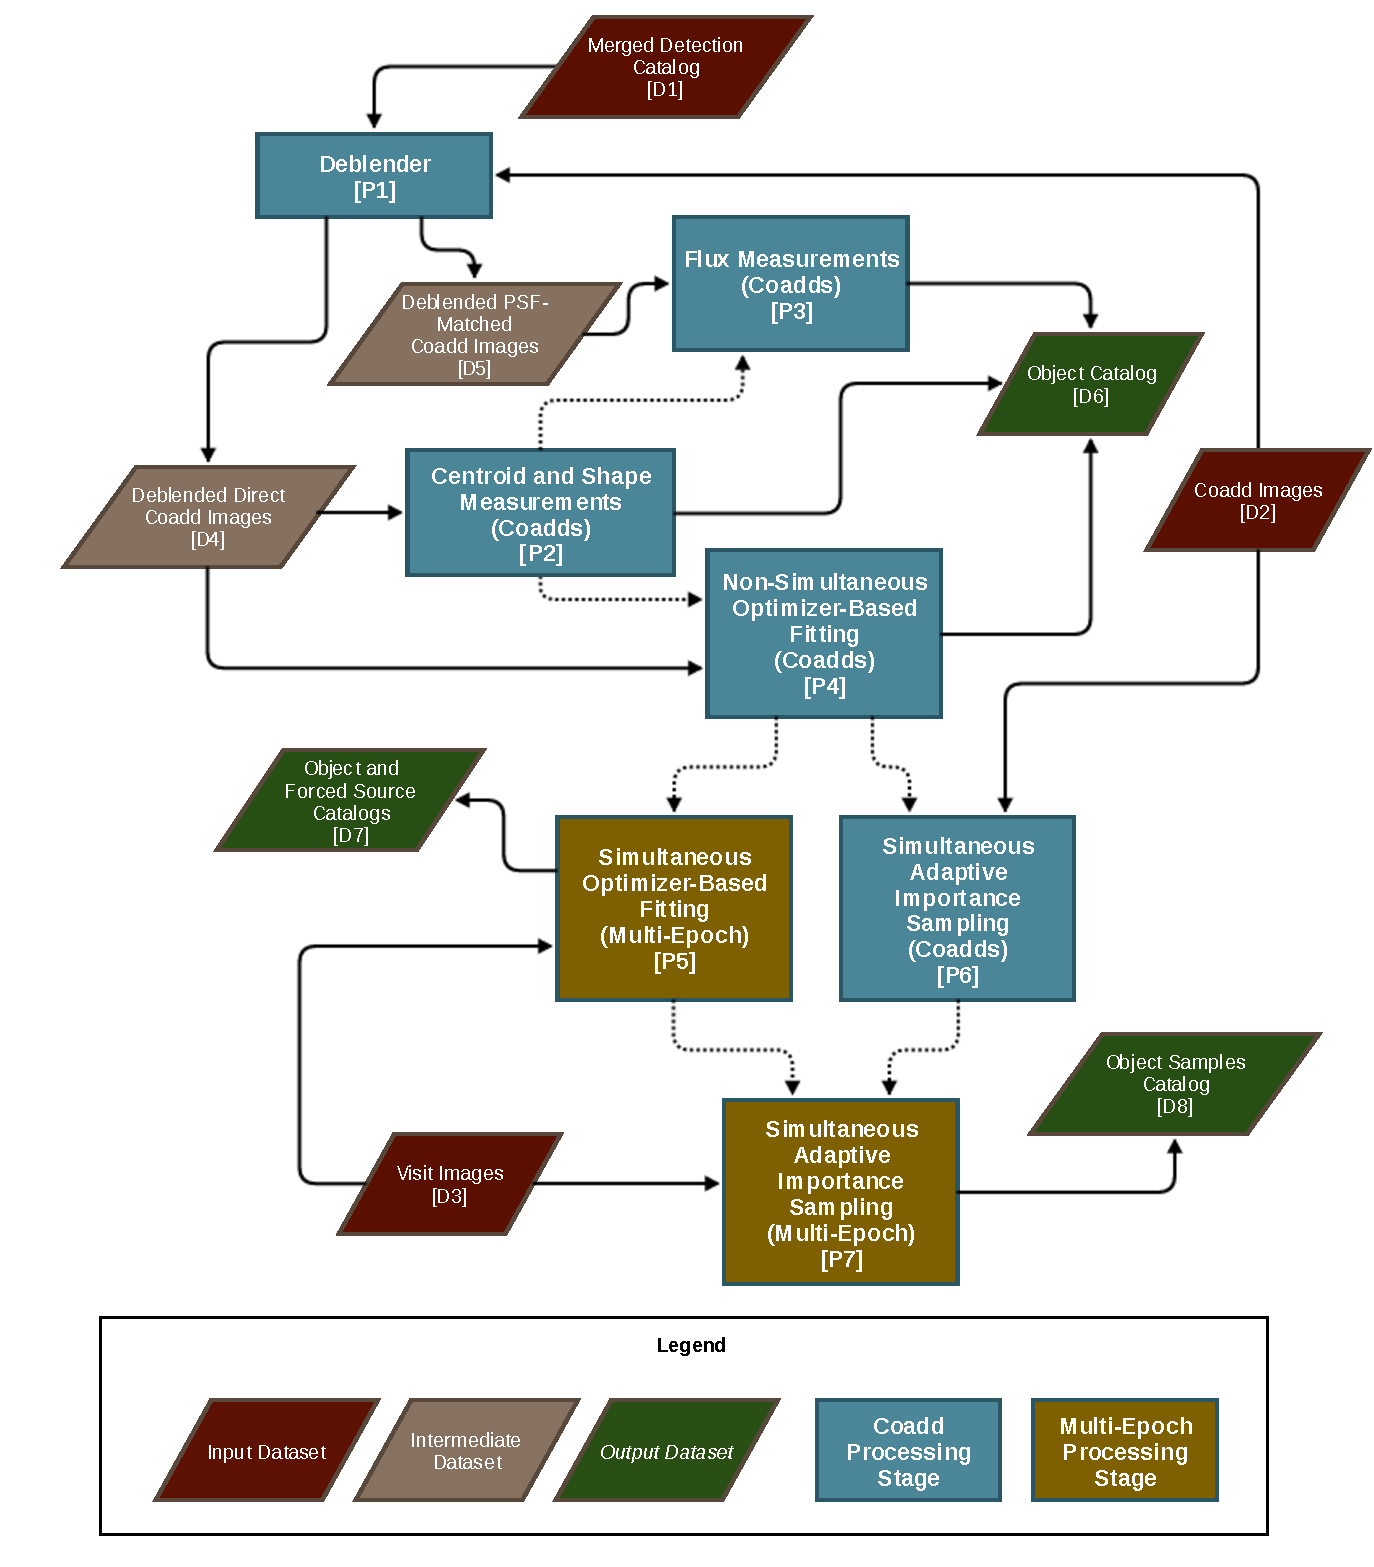
\includegraphics[width=\columnwidth]{flowchart}
\caption{Baseline Pipeline for Blended Measurement}
\label{fig:flowchart}
\end{figure}

\subsection{Baseline}

The first major processing stage described here is the Deblender [P1], which
we imagine as an algorithm very similar to that the SDSS {\em Photo} deblender
described in Section~\ref{sec:deblender}, likely using a symmetry ansatz to
define templates.  The inputs will be a detection catalog containing merged
{\texttt Footprints} and {\texttt Peaks} from all detection images [D1], and
at least one coadd image per filter [D2].  We may have multiple input coadds
for each filter, representing different depth vs. resolution tradeoffs or
different epochs, and possibly some coadds that represent combinations of data
from different filters. The details of these inputs and the parallelization
and data flow within the deblender itself are beyond the scope of this
document. The outputs are deblended pixel values for both direct [D4] and PSF-
matched [D5] coadds (generated by sequentially replacing neighbors with noise,
as described in Section~\ref{sec:deblender}).

These deblended coadds are used for three different groups of measurement
algorithms, which we split here into separate processing stages mostly for
clarity in their inputs and outputs (they may be run together):
\begin{itemize}
\item We start with centroid and moments-based shape measurements [P2] on
    deblended direct coadds [D4].  This includes all the standard centroiders
    as well as adaptive second moments.  For each centroid or shape
    measurement, we'll define a single cross-filter output, either by
    selecting one filter (or combination of filters) as canonical or using
    algorithms that make use of all data from all filters.
\item These consistent cross-filter centroid and shape measurements are used
    as inputs for traditional flux measurements [P3] on deblended PSF-matched
    coadds [D5].  These will include at least a sequence of aperture fluxes at
    predetermined radii as well as Kron and Petrosian fluxes.
\item We'll also fit galaxy models [P4] to the deblended direct coadd
    images~[D4] (fitting each object separately, of course, since these are
    deblended pixel values).  Because the galaxy models become point sources
    at the zero radius limit, and there's no variability or astrometric
    information on the coadd, there'd be no point to additionally fitting a
    moving and/or variable point source model at this stage.  We'll do at
    least one fit that uses the same structural (non-amplitude) parameters
    in all filters, to allow the model fluxes to be useful as for galaxy
    colors (see \ref{sec:consistent-galaxy-colors} for an alternative).  We
    may also perform completely independent model fitting each each filter.
\end{itemize}

All three measurement stages will have some outputs that are included in the
final object catalog [D6], but some may have temporary outputs that are used
only to feed other measurement stages (indicated by the dotted lines in
Figure~\ref{fig:flowchart}).  At this level of detail, we consider each of
these measurements to have access to coadds from all filters, to allow forced
measurements in one filter that depend on non-forced measurements in another.
Whether this is done by giving algorithms access to all filters simultaneously
or processing filters in serial (possibly more than once) is beyond the scope
of this paper.

The last stage of measurement on coadds is simultaneous Monte Carlo sampling
[P6], on the original (not deblended) direct coadds [D2].  We will again use
galaxy models here, though they may not be the same as those used in [P4].
The outputs from this stage are used only as inputs to a multi-epoch
sampling step [P7], and are essentially just a performance optimization.

In multi-epoch mode, we use hybrid models (as described in
Section~\ref{sec:model-selection}) and consider all objects in a blend
simultaneously, first fitting with an optimizer [P5] and then Monte Carlo
sampling [P7].  In both cases we will fit to multiple filters simultenously
(though perhaps not all filters), and only allow the flux to vary between
filters (i.e. the models will not support variability -- but see also
\ref{sec:variable-models} for an alternative).  As in the coadd fitting, the
structural parameters of the galaxy models will be required to be the same in
each filter.  The most important use case for the Monte Carlo samples [D8] is
shear estimation for gravitational lensing, but we anticipate it being useful
for any study of faint objects for which unbiased population statistics are
more important than precise measurements of individual objects.  The
optimizer-based fitting is should produce our best astrometric measurements
for fainter stars, and may yield better galaxy photometry and morphology
measurements than the deblended coadd fitting.

The simultaneous optimizer-based fit will also be used as templates for
another round of deblending (as in Section~\ref{sec:models-as-templates}),
this time producing deblended pixel values for individual visits [D7].  These
will be used for forced PSF photometry at the per-epoch positions determined
from the simultaneous multi-epoch fit.  This will populate the forced source
catalog [D9], which represent our best estimates of the lightcurves of
faint variable objects.  We use positions from multi-epoch fitting to
consistently handle stars with significant proper motions, and we perform only
PSF photometry, as the vast majority of variable objects are indeed point
sources.

For all multi-epoch measurements, we include models for transient and fast-
moving objects detected in difference images [D10], as described in
Section~\ref{sec:time-domain}. These models will have a free flux
parameter in each epoch, but will have centroids fixed at the position
determined from detection image(s).

\subsection{Possible Modifications}
\label{sec:alternatives}

\subsubsection{Likelihood Coadds}

\label{sec:likelihood-coadds}

Likelihood coadds (also known as Kaiser coadds or detection maps) present an
intriguing but untested alternative to direct coadds.  They represent an
optimal combination of images in both image quality and S/N (impossible with
direct coadds), but cannot be interpreted in the same way as traditional
coadds and single-epoch images, requiring completely new algorithms for all
operations performed on them.  As a result, making use of likelihood coadds
may require considerably more human effort, but it could reduce the need for
multi-epoch processing (but probably not eliminate it). If they prove viable,
likelihood coadds would replace direct coadds in most or all of the places the
latter are currently used.

\subsubsection{Model Fluxes on PSF-Matched Coadds}

\label{sec:models-on-psf-matched-coadds}

Forward fitting of galaxy models only formally accounts for differences in PSF
size across filters when the galaxy model is flexible enough to capture the
true morphology of the galaxy being fit -- a condition that is never fully
met in practice.  The best galaxy colors may thus require fitting to
PSF-matched coadds instead of direct coadds, even though direct coadds may
allow the model parameters to be constrained better.

If fitting to PSF-matched coadds produces better galaxy colors, we will do
this in addition to fitting on direct coadds, as the latter will still produce
better estimates of structural parameters and a better starting point for
Monte Carlo sampling.

\subsubsection{Consistent Cross-Filter Galaxy Structural Parameters}

\label{sec:consistent-galaxy-colors}

Galaxies do not have the same morphology in each filter, but the differences
between wavelengths are typically subtle enough that colors have historically
been measured using the same structural parameters in each filter. If the PSF
is also the same in each filter, this guarantees a consistent color even if
the morphology is not correct in any of the filters, because it selects the
same (incomplete) subset of the galaxy's light in each filter.

It may also be possible to use more flexible models in which the structural
parameters can vary between filters to produce a better estimate of the total
flux of the galaxy (and colors from the total fluxes are of course consistent
as well).  This requires additional degrees of freedom in the fit, and the
additional flexibility increases the danger that measurements will select an
inconsistent subset of the galaxies light across filters.  If we can provide
external constraints on how much the structural parameters can vary between
filters (e.g. via Bayesian priors trained on space-based data), we may be able
to allow for these extra degrees of freedom in a realistic way, which should
produce better total flux and morphology estimates as well as consistent
colors.  These colors may also be higher S/N than those measured using the
same model across filters on PSF-matched coadds; this depends on how
the extra degrees of freedom from including more parameters compares to the
loss of information in PSF-matched coadds.

\subsubsection{Variability in Multi-Epoch Modeling}

\label{sec:variable-models}

Our baseline plan for multi-epoch modeling assumes objects have the same flux
in every epoch.  This is obviously incorrect for many point sources and even
some galaxies (due to low-level AGN), and we may produce better results by
including variability in these models.  Such models could produce better
measurements of light curves than simple forced photometry (perhaps making a
separate forced photometry stage unnecessary). They could also improve
star/galaxy classification of blended objects, and hence blended overall,
by applying the ansatz that flux that varies between epochs should be
attributed to point sources.

The main problem with introducing variability into the models is that it
introduces many more degrees of freedom into the fit, vastly increasing the
dimensionality of the problem.  Given the many types of variable objects, and
the complexity of the light curves of any of these, it is essentially
impossible to devise analytic models that could predict the flux from just a
few parameters; it will almost certainly be necessary to include an additional
amplitude parameter for each epoch being fit.  Because the model is linear in
these parameters, however, their likelihood with all other parameters held
fixed is exactly Gaussian, and this may enable us to marginalize analytically
over these amplitudes while exploring the rest of the parameter space, while
still retaining enough information to reconstruct the full joint distribution.
This will require defining a Bayesian prior on the vector of amplitudes,
though this could be based simply on the deviation from the mean flux rather
than the distribution of fluxes as a function of time.

The simplest way to include variability in the models is to just add
one amplitude parameters to the hybrid model when it is in moving-point source
mode.  This doesn't fully account for galaxies with AGN, however:
\begin{itemize}
\item In cases where the AGN flux dominates the total galaxy flux (i.e.
    quasars), this model would likely prefer a moving point-source model,
    ignoring extended flux from the galaxy even if it was detectable.
\item In cases where the extended flux is comparable to or dominant over the
    AGN, these models would likely prefer the non-variable galaxy model, and
    treat the variability as noise.  Because this ``noise'' would be
    inconsistent with the noise model we use to construct the likelihood, our
    any estimates of goodness-of-fit.  Of course, this is also what happens
    (on a larger scale) when none of our models include variability.
\end{itemize}
A potential solution this problem would be to use a hybrid model that is a
linear combination of a variable moving point source and static galaxy model,
rather than hybrid model that transitions between the two.  While this would
have the same number of parameters overall, it would have more active at any
time, truly increasing the dimensionality of the fit, though it would
simplify the topology of that space significantly.  More importantly, it would
require the computationally expensive evaluation of a galaxy model for all
likelihood evaluations, even when the evidence strongly suggests a point
source.  As a result, this approach is probably not feasible unless we can
devise a clever way to speed up or avoid some of those model evaluations.

While variable models may or may not be used in the mainline processing, it
will be necessary to implement the capability to fit them regardless, and not
just to evaluate them for use in the mainline processing -- this sort of
modeling is likely to be an important category of Level 3 processing, as any
science involving strongly lensed quasars or AGN in galaxy clusters will
require modeling complex blends of variable point sources and galaxies.

\subsubsection{Forced Photometry on Difference Images}

\label{sec:diffim-forced-phot}

Another way to improve blended measurement of variable sources could be to run
forced photometry on difference images instead of the original visit images.
Because the extend light from galaxies is static, this should reduce the
complex deblending problem to an exactly-solvable problem involving only
point sources.

The only problem with this approach is the additional complexity in
understanding the image data: the noise properties and effective PSF of a
difference image are much more complex than that of a single epoch image, as
we probably can't afford to simply ignore contributions from the template
image.

This approach probably has the highest ceiling of any method for measuring
variable blended sources, but it is untested and the mathematical formalism
has yet to be developed.

\subsubsection{Deblend Template Translation}

\label{sec:deblender-translation}

Instead of using the models produced by simultaneous fitting as deblend
templates for forced photometry, it may be possible to ``translate'' the
deblend templates produced on the coadds to individual visit images.  This
translation would involve reconvolving to a different PSF (which will be a
deconvolution for some images), and transforming to a new coordinate system.
In fact, some sort of deblend translation code will have to exist even if we
do not take this approach for forced photometry, in order to construct
consistently-deblended direct and PSF-matched coadds (though that translation
would involve only convolution to a larger PSF, assuming the deblending is
done originally on direct coadds).

Transformation to a new coordinate system is just a matter of resampling, but
reconvolution to a new PSF is trickier, at least when deconvolution may be
involved.  One possibility would be to use the same matching kernel algorithms
used to build difference image; while these do not perform as well when
matching a large PSF to a smaller one, they can deconvolve to a small degree.

We could also use regularized deconvolution techniques (e.g. sparse wavelet
transforms) to construct deconvolved templates (still using symmetry arguments
rather than analytic models), and then convolve them with the appropriate PSF
for the image to be deblended, whether that's a coadd or a single-epoch image.
A key point in this approach is that the deblended template need not match the
true deconvolved source morphology (though clearly that is advantageous), or
even be related to the pixel data in any statistically rigorous way; any
template that, when convolved with the PSF, approximates the as-observed
morphology could work.

Translated deblending has the potential to better capture galaxy morphology
than the simultaneous fitting approach we propose as the baseline, simply
because the translated deblend templates will have more flexibility than the
analytic models used in fitting.  On the other hand, translated deblend
templates will be limited by the quality of the coadd and their inability to
account for proper motions.

\end{document}
